\chapter{Exporting geometry from Salome to OpenFOAM}
\thispagestyle{empty}
\label{sec:chap12}
\newcommand{\LocCHtwelvefig}{\Origin/CHAPTERS/chap12/figures}

A 90 deg pipe bend is perhaps the most frequent used fitting in piping systems. The pressure losses in such bends are therefore of considerable engineering importance. This chapter is extension of the the chapter number, where we learnt about creating and meshing a curved pipe in Salome, hence it is manditory that the learner should have already gone through the previous chapter . In this chapter we will learn how to group the mesh faces in Salome, save the mesh file and export the mesh file to be used in OpenFOAM. Here we will also create a case directory to solve this problem and visualize the results in Paraview. \newline

Open the salome working window as shown in the previous chapters. Click on the File in the menu bar and click on Open. Now go to the path where you had saved your geometry in the previous chapter i.e. \textbf{"$*$.hdf"} and open it. \\

Since we have already meshed our geometry will will skip the geometry module and select the Mesh module from module drop down menu. Module $>>$ Mesh. In the object browser we can see the Mesh module, click it to expand the Mesh module tree. Here we will see Mesh$\_$1. The meshed geometry will not be visible in the Salome working window. To view the meshed geometry , right click on Mesh$\_$1 and click on Show. The meshed geometry can be seen as shown in figure, \ref{mesh_1}. Once we open the mesh we will start to group it so that we can export it and use this in OpenFOAM. 

\begin{figure}[h]  
\centering
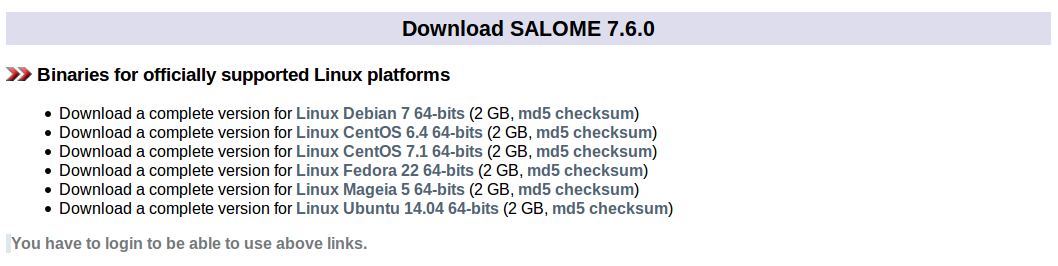
\includegraphics[scale=0.35]{\LocCHtwelvefig/mesh_12_1.png}
\caption{Meshed geometry in Salome working window}
\label{mesh_1}
\end{figure}   

\section{Creating Groups}

In Mesh we can create a group of elements of a certain type. This helps us to identify the boundary patches in OpenFOAM. To create group from the top menu bar click on "Mesh" and slect "Create Group" To create a group once needs to define the following, \newline
\begin{itemize}
\item Mesh - The mesh from which elements will be selected to form the group. We can select the mesh in the Object Inspector Menu or in the 3D viewer.
\item Element type - These are a set of radio buttons which allows us to select the type of element which will form the group.
\begin{itemize}
\item Nodes
\item 0D elements
\item Ball
\item Edges
\item Faces
\item Volumes
\end{itemize}
\item Name - this field allows you to enter the name of the new group eg, "inlet"
\item Color - assigns color to a certain group. This helps to display the elements of a group
\item We can also distinguish between three group type as Standalone geometry, Group on geometry and group on filter.
\end{itemize}
 
\section{Grouping Mesh}
Since we have three patches in our geometry we will select the "Face" option from create groups and Group on geometry as the group type, this is because we will be grouping the elements of a certain type generated on our geometry. The Group on Geometry can be created only if the mesh is based on geometry. To define a group we choose the Group on geometry check box and then click the selection button besides Gemetrical object as shown in the figure \ref{mesh_1}. 

\begin{figure}[h]  
\centering
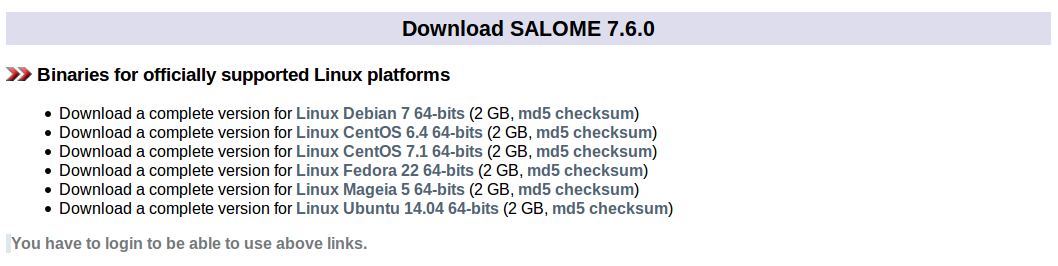
\includegraphics[scale=0.35]{\LocCHtwelvefig/mesh_12_1.png}
\caption{Meshed geometry in Salome working window}
\label{mesh_1}
\end{figure} 

Here we get two options
\begin{itemize}
\item Direct geometry selection - to select a shape in the Object Browser 
\item Find geometry by mesh element selection - to activate a dialog which retrives a shape by the selected element generated on this shape.
\end{itemize} //

We will use direct geometry selection since we have already grouped our geometry while creating the geometry. Open the geometry tree in the object browser and click on the Pipe$\_$1 and select the group which we had created during geometry such as "inlet", "outlet" and "walls". These faces can be identified by color by selecting a color from Color group . We can give names to this group of our choice , in this chapter we have kept the same name as that given in geometry i.e. "Inlet".Finally click on Apply and close to end the geometry selection. Follow the similar procedure for naming outlet faces of the mesh. Inlet and Outlet group will be seen in the Mesh-1 tree. For selecting the faces for walls we select the element type in Create group as Face and Group type as Group on Filter. Now we click on the set filter.This open a new box named as Filter for faces \ref{mesh_1}, click on the "Add" button. In the drop down menu below Criterion select "Free faces" and click on Apply and close. You can provide any color of your choice here. Click on Apply and close to create Group-1. From the menu bar now click on Mesh menu and select Cut of groups and select the main object as Group-1 as shown in figure \ref{mesh_1}. Click on tool object and from grouped object select Inlet, hold the shift key and select Outlet. We can see the Result name on top of the window, type "walls". Select any color of your choice and click on Apply and close. This will now create a group named "walls" in the Mesh tress in object browser. Delete the Group-1 in the mesh tree as we no longer need the group. We can save our work by clicking on the Save Document option just above object browser. To export the mesh file right click on Mesh-1 and select Export and click on UNV file. Name this file as "bentpipe" and save it in your working directory. Now we can close salome.

\section{Creating Case directory}

To solve this problem in OpenFOAM we need to first create a case directory in OpenFOAM. We will be using icoFoam solver to solver this problem, which is an incompressible transient solver for laminar flows. We create a directory inside icoFoam and name it as bentpipe. Copy the bentpipe.unv file which we had saved and paste this into the bentpipe folder. Now Copy the 0 and system folder from the cavity folder to the bentpipe folder. The directory structure of the bentpipe folder is as shown in the figure, \ref{mesh_1}.

\begin{figure}[h]  
\centering
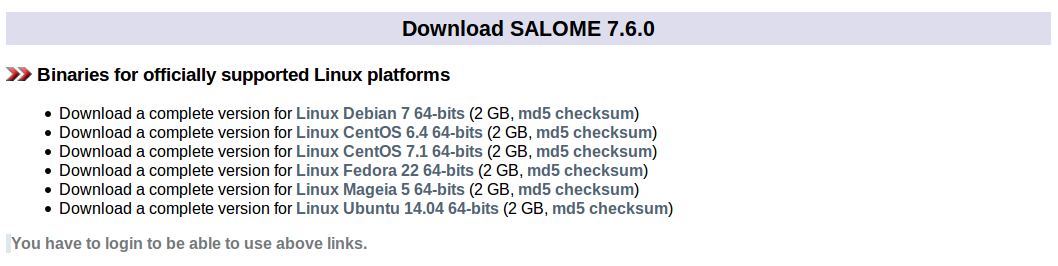
\includegraphics[scale=0.35]{\LocCHtwelvefig/mesh_12_1.png}
\caption{Meshed geometry in Salome working window}
\label{mesh_1}
\end{figure}

Note that, we have not copied the constant folder here as it will be created once we have converted our mesh file from UNV to Foam format. Open the terminal window and type the path for bentpipe inside the icoFoam solver as follows \\
/OpenFOAM/OpenFOAM-2.x.x/tutorial/incompressible/icoFoam/bentpipe \\

\subsection{Geometry conversion}

To convert the geometry from UNV format to OpenFOAM recognisable format we use the command as shown below, \\

ideasUnVToFoam -filename \\

The file name in our case would be bentpipe.unv. Once the file is converted we can see that the constant folder is created. The polyMesh folder inside constant folder stores the information regarding geometry, check this folder for files such boundary, faces, neighbours, owner, points. Also do not forget to copy the transportProperties file from the cavity folder and paste this inside the constant folder

\subsection{Geometry Scaling}     

In Salome, by default the geometry is created in millimeters. To convert the geometry from millimeters to centimeters we will use the OpenFOAM utility of transformPoints. In In the command terminal type  the command given below for using this utility and press enter\\

transformPoints -scale '(0.01 0.01 0.01)' \\

We will see that the geometry has been converted to centimeters.

\section{Setting 0 folder}

As we had copied the 0 folder from the cavity case we need to make changes inside the pressure (p) and Velocity (U) file for matching the boudnary names given in Salome. Open each file and insert the boundary name and boundary condition as shown in the table below for both pressure and velocity.


\section{Visualization}

The case directory tress for the bentpipe case will be as shown below, \ref{mesh_1}.

\begin{figure}[h]  
\centering
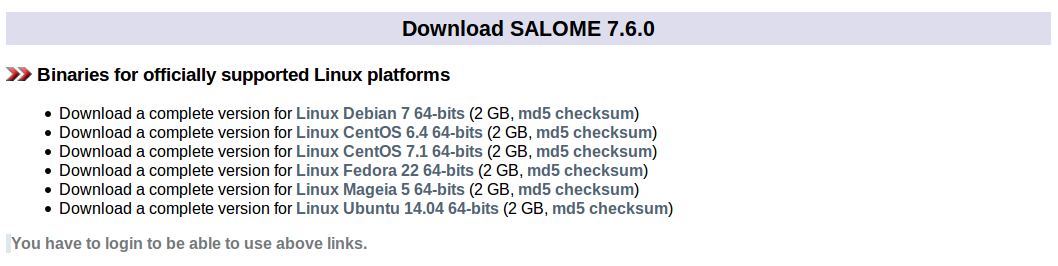
\includegraphics[scale=0.35]{\LocCHtwelvefig/mesh_12_1.png}
\caption{Meshed geometry in Salome working window}
\label{mesh_1}
\end{figure}

To visualize the geometry we will open Paraview using the paraFoam command in terminal.Click on Apply button in the Object Inspector menu, we will see the geometry as seen in the figure \ref{mesh_1}.

\begin{figure}[h]  
\centering
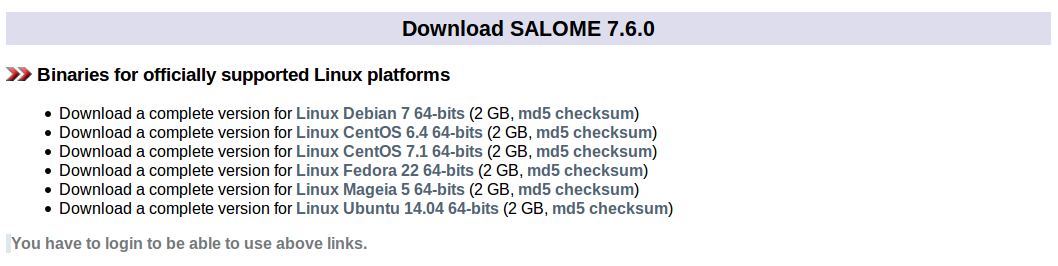
\includegraphics[scale=0.35]{\LocCHtwelvefig/mesh_12_1.png}
\caption{Meshed geometry in Salome working window}
\label{mesh_1}
\end{figure}

Now to view the mesh , from the drop down menu select Surface with Edges. Zoom into the geometry to see the mesh. In Mesh parts inside Object Inspector we can see that the groups have been properly created and match with that created in Salome namely "Inlet", "Outlet" and "Walls". Volume of pipe by default is named as "internalMesh". This bring us to the end of this chapter.

\section{Assignment}

In this chapter and the earlir chapter 11, we have seen how to create geometry, mesh the geometry and create groups for the mesh file to be imported inside OpenFOAM. As an assignment create a bentpipe with radius 5 mm and total length of 300 mm and export the geometry in "unv" file format. Finally visualize the results in OpenFOAM.

